% !TEX encoding = UTF-8
% !TEX TS-program = pdflatex
% !TEX root = ../tesi.tex

%**************************************************************
\chapter{Progettazione e codifica}
\label{cap:progettazione-codifica}
%**************************************************************

%**************************************************************
\section{Tecnologie usate}
\label{sec:tecnologie-strumenti}

Per la realizzazione del progetto di stage è stato dedicato diverso tempo all'apprendimento delle tecnologie e linguaggi richiesti, di seguito elencati.

\subsection{Linguaggi di programmazione}

\subsubsection{PHP}
PHP (acronimo ricorsivo di "PHP: Hypertext Preprocessor") è un linguaggio di \textit{scripting} interpretato, originariamente concepito per la programmazione di pagine web dinamiche. L'interprete PHP è un software libero distribuito sotto la PHP License.
\\
Attualmente è principalmente utilizzato per sviluppare applicazioni web lato server, ma può essere usato anche per scrivere script a riga di comando o applicazioni \textit{stand-alone} con interfaccia grafica.
\\
\begin{figure}[!h] 
    \centering 
    
\includegraphics[width=4cm]{immagini/loghi/php.png}
    \caption{Logo PHP}
\end{figure}

\subsubsection{JavaScript}
JavaScript è un linguaggio di \textit{scripting} orientato agli oggetti e agli eventi, comunemente utilizzato nella programmazione Web lato \textit{client} per la creazione, in siti web e applicazioni web, di effetti dinamici interattivi tramite funzioni di script invocate da eventi innescati a loro volta in vari modi dall'utente sulla pagina web in uso.
\begin{figure}[!h] 
    \centering 
    
\includegraphics[height=3cm]{immagini/loghi/javascript.png}
    \caption{Logo JavaScript}
\end{figure}

\subsubsection{AJAX}
AJAX, acronimo di Asynchronous JavaScript and XML, è una tecnica di sviluppo software per la realizzazione di applicazioni web interattive (Rich Internet Application). Lo sviluppo di applicazioni HTML con AJAX si basa su uno scambio di dati in background fra web browser e server, che consente l'aggiornamento dinamico di una pagina web senza esplicito ricaricamento da parte dell'utente.
\begin{figure}[!h] 
    \centering 
    
\includegraphics[width=3cm]{immagini/loghi/ajax.png}
    \caption{Logo AJAX}
\end{figure}
AJAX è asincrono nel senso che i dati extra sono richiesti al server e caricati in background senza interferire con il comportamento della pagina esistente. Normalmente le funzioni richiamate sono scritte con il linguaggio JavaScript. Tuttavia, e a dispetto del nome, l'uso di JavaScript e di XML non è obbligatorio, come non è detto che le richieste di caricamento debbano essere necessariamente asincrone.

\subsubsection{HTML 5}
L'HTML5 è un linguaggio di \textit{markup} per la strutturazione delle pagine web, pubblicato come \textit{W3C Recommendation} da ottobre 2014.
\\
\begin{figure}[!h] 
    \centering 
    
\includegraphics[height=3cm]{immagini/loghi/html.png}
    \caption{Logo HTML5}
\end{figure}
\\
Gli obiettivi di HTML5 sono di migliorare il linguaggio con il supporto agli ultimi file multimediali ed altre \textit{features}; di mantenere il linguaggio sia leggibile dagli umani che consistente tra i vari dispositivi e browser, abbandonando la rigidità dell'XHTML, rimanendo retrocompatibile con i software più vecchi.


\subsubsection{CSS 3}
Il CSS (acronimo di Cascading Style Sheets), in informatica, è un linguaggio usato per definire la formattazione di documenti HTML, XHTML e XML ad esempio i siti web e relative pagine web. Le regole per comporre il CSS sono contenute in un insieme di direttive (Recommendations) emanate a partire dal 1996 dal W3C.
\\
\begin{figure}[!h] 
    \centering 
    
\includegraphics[height=3cm ]{immagini/loghi/css.png}
    \caption{Logo CSS3}
\end{figure}
\\
L'introduzione del CSS si è resa necessaria per separare i contenuti delle pagine HTML dalla loro formattazione e permettere una programmazione più chiara e facile da utilizzare, sia per gli autori delle pagine stesse sia per gli utenti, garantendo contemporaneamente anche il riutilizzo di codice ed una sua più facile manutenzione.


\subsubsection{SQL}
In informatica SQL (Structured Query Language) è un linguaggio standardizzato per database basati sul modello relazionale (RDBMS) progettato per:
\begin{itemize}
    \item creare e modificare schemi di database;
    
    \item inserire, modificare e gestire dati memorizzati;
    
    \item interrogare i dati memorizzati;
    
    \item creare e gestire strumenti di controllo e accesso ai dati.
\end{itemize}
\begin{figure}[!h] 
    \centering 
    
\includegraphics[width=4cm]{immagini/loghi/sql.jpg}
    \caption{Logo SQL}
\end{figure}
\newpage
%**************************************************************
\subsection{Frameworks e PlugIn}

\subsubsection{Framework aziendale}
    Di seguito uno schema del \textit{filesystem} di un progetto web sviluppato con il \textit{framework}:
    \begin{figure}[!h] 
        \centering 
        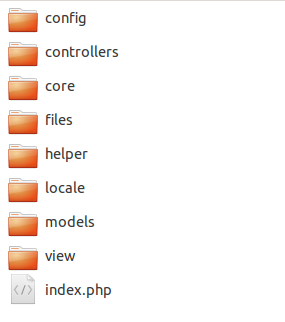
\includegraphics[width=4cm]{immagini/f12doc/a.png}
        \caption{Esempio di \textit{filesystem}}
    \end{figure}
    I Componenti principali del \textit{framework} saranno i seguenti:
        \begin{itemize}
            \item \textbf{Router:} il \textit{router} si trova all'interno della cartella core ed è una classe che si occupa di rimappare le richieste HTTP a chiamate alle azioni dei \textit{controller}. Inizialmente implementeremo un \textit{router} nel quale andranno registrate esplicitamente le mappature tra URL e azioni; successivamente estenderemo il concetto ed implementeremo un \textit{router} che analizzerà determinate directory del \textit{filesystem} per recuperare, in base all'URL richiesto, il \textit{controller} corretto;
            
            \item \textbf{Controller:} si trovano all'interno della cartella \textit{controllers} e rappresentano un insieme di azioni che potrebbero essere intraprese dall'utente. Ogni azione verrà rappresentata da un metodo definito nelle classi che estenderanno \textit{controller}; i metodi verranno richiamati in base a determinate condizioni e dovranno restituire una stringa che verrà inviata in output all'utente (solitamente una View renderizzata);
            
            \item \textbf{Models:} si trovano dentro la cartella models e si occupano dell'interfacciamo con il database. All'interno di models vengono fatte le query ed estratti i dati che poi verranno passati ai \textit{controller} e di conseguenza alle view. Solo dai \textit{controller} è possibile richiamare i metodi implementati all'interno dei models;
            
            \item \textbf{View:} si trovano nella cartella view e sono responsabili di visualizzare i dati dei modelli direttamente all'utente aggiungendo della grafica e del testo che rendano comprensibili i dati visualizzati;
            
            \item \textbf{Template:} rappresenta un template che verrà utilizzato come contenitore per renderizzare i dati assegnati in fase di costruzione;
            
            \item \textbf{Helper:} sono delle \textit{utility} utilizzate dalle view per poter formattare i dati presentati all'utente finale.
        \end{itemize}
    Esempio di richiesta http del \textit{framework}:
    \begin{figure}[!h] 
        \centering 
        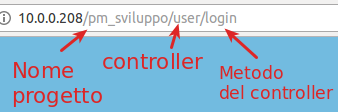
\includegraphics[width=8cm]{immagini/f12doc/b.png}
        \caption{Esempio di richiesta http}
    \end{figure}
    Ogni richiesta http che arriva al \textit{framework} contiene tutte le informazioni necessarie a renderizzare la pagina richiesta. Il \textit{router} si occupa di interpretare la richiesta php e scomporla per poter inizializzare l'opportuno \textit{controller} (nell'esempio stiamo invocando il \textit{controller} user) e invocare il metodo richiesto.
    \\
    L'esempio sopra riportato mostrerà la pagina di login del \textit{framework}.

\subsubsection{Bootstrap}
Bootstrap è una raccolta di strumenti liberi per la creazione di siti e applicazioni per il Web.
\begin{figure}[!h] 
    \centering 
    
\includegraphics[width=4cm]{immagini/loghi/bootstrap.png}
    \caption{Logo Bootstrap}
\end{figure}
\\
Contiene modelli di progettazione basati su HTML e CSS, sia per la tipografia,
che per le varie componenti dell'interfaccia, come moduli, pulsanti e navigazione,
così come alcune estensioni opzionali di JavaScript. Inizialmente si presentava come un progetto interno a Twitter, ma successivamente è diventato indipendente ed è perciò utilizzabile liberamente dagli sviluppatori come base per la realizzazione di interfacce web. Al momento è considerato il più efficiente ed il più utilizzato framework per rendere i siti web responsive. La versione usata nel progetto è Bootstrap 3.

\subsubsection{JQuery}
jQuery è una libreria JavaScript per applicazioni web. Nasce con l'obiettivo di semplificare la selezione, la manipolazione, la gestione degli eventi e l'animazione di elementi DOM in pagine HTML, nonché implementare funzionalità AJAX.
\\
Le sue caratteristiche permettono agli sviluppatori JavaScript di astrarre le interazioni a basso livello tra interazione e animazione dei contenuti delle pagine. L'approccio di tipo modulare di jQuery consente la creazione semplificata di applicazioni web e versatili contenuti dinamici.
\begin{figure}[!h] 
    \centering 
    
\includegraphics[width=4cm]{immagini/loghi/jquery.png}
    \caption{Logo JQuery}
\end{figure}
\\
È un software libero, distribuito sotto i termini della Licenza MIT e nel 2018, jQuery risulta la libreria JavaScript più utilizzata su Internet.

\subsubsection{DataTables}
Realizzato come plugin di jQuery, DataTables trasforma una comune tabella HTML aggiungendo tutte le caratteristiche richieste. DataTables utilizza il principio detto del \textit{progressive enhancement}, ossia se per qualche ragione il javascript non viene caricato, la tabella viene comunque resa in HTML standard ed è quindi pienamente fruibile.
\\
L'utilizzo delle DataTables è dovuto alla necessità di dover creare, all'interno pagine web, delle tabelle di dati interattive: filtrabili, ordinabili e paginate.

\subsubsection{EasyAutocomplete}
Una delle caratteristiche più utili e apprezzate per un motore di ricerca è sicuramente la sua capacità di offrire dei suggerimenti a chi effettua una ricerca.
\\
Una libreria molto completa e semplice da usare è EasyAutocomplete. Supporta suggerimenti da locale o remoto in \emph{JSON}\glsfirstoccur, \emph{XML}\glsfirstoccur e \textit{plain text}. 
Si fa apprezzare anche per la chiarezza della documentazione oltre alla semplicità di utilizzo essendo un \emph{plugin}\glsfirstoccur di jQuery.
\\
Di seguito viene riportato un esempio di \textit{script} realizzato da me per offrire all'utente tutte le possibilità di proprietario di protocollo in base alla tipologia selezionata.
\label{EasyAutocomplete}
\begin{lstlisting}[language=HTML, caption=HTML per \textit{EasyAutocomplete}]
    <div class="row">
        <div class="col-md-6">
            <div class="form-group form-reg">
                <label for="tipologia-intestatario">Tipologia proprietario</label>
                    <select class="form-control tipo-prop required" id="tipo-prop" name="tipo_proprietario">
                        <option></option>
                        <option value="C">Cliente</option>
                        <option value="F">Fornitore</option>
                        <option value="K">Contatto</option>
                        <option value="N">Nuovo Contatto</option>
                    </select>
                </div>
            </div>
            <div class="col-md-6">
                <div class="form-group form-reg">
                    <label for="nome-intestatario">Nome proprietario</label>
                    <input class="form-control general-autocomplete nome-proprietario" id="upper" extra-params="tipo-prop" data-url="<?php echo SITE_ROOT?>/protocolli/getSco"  name="nome_proprietario" disabled>
                </div>
            </div>
        </div>
    </div>
\end{lstlisting}
\begin{lstlisting}[language=Java, caption=JavaScript per EasyAutocomplete]
$('.general-autocomplete').each(function (){
    var dataType = 'json';
    var minLength = 2;
    var appendTo = '#container';
    var extraParams = '';

    if($( this ).attr('data-type'))
        dataType = $( this ).attr('data-type');

    if($( this ).attr('min-length'))
        minLength = $( this ).attr('min-length');

    if($( this ).attr('append-to'))
        appendTo = $( this ).attr('append-to');

    var url = $( this ).attr('data-url');

    var existextraparam = false;
    if($( this ).attr('extra-params'))
        existextraparam = true;

    var input = $(this);


    $( this ).autocomplete({
        source: function(request, response) {
            $.ajax({
                url: url+ (existextraparam ? componiurl(input.attr('extra-params')) : ''),
                dataType: "json",
                data: {
                    term : request.term
                },
                success: function(data) {
                    response(data);
                }
            });
        },
        type: "POST",
        minChars: minLength,
        dataType: dataType,
        data: {'tipo':$('#tipo-prop').val()},
        onSearchStart: function (query) {
            showOverlay();
        },
        onSearchComplete: function (query, suggestions) {
            hideOverlay();
        }
    });
});

function componiurl(idparam) {
    return '?' + $('#'+idparam).attr('name') + '=' + $('#'+idparam).val();
}
\end{lstlisting}
\newpage

%**************************************************************
\subsection{Formato per l'interscambio di dati}
\subsubsection{Array}
Un array può essere considerato come una collezione di elementi ognuno identificato da un indice; gli indici di un array possono essere numerici o stringhe. Gli elementi dell'array possono contenere al proprio interno qualsiasi tipo di dato, compresi oggetti o altri array.
\\
Grazie a quanto detto un metodo valido ed intuitivo per l'interscambio di dati è quello mediante array.
\subsubsection{JSON}
JSON ("JavaScript Object Notation") è un formato di scambio dati leggero e facile da leggere e scrivere per le macchine e di non difficile interpretazione per gli umani.
\begin{figure}[!h] 
    \centering 
    
\includegraphics[width=6cm]{immagini/loghi/json.png}
    \caption{Logo JSON}
\end{figure}
\\
Si basa su un sottoinsieme del linguaggio di programmazione JavaScript, anche se ne è indipendente, ed inoltre è un formato di testo completamente indipendente da qualsiasi linguaggio. Per queste caratteristiche è un linguaggio di scambio dati ideale. 
\\
JSON è costruito su due strutture:
\begin{itemize}
    \item una collezione di coppie nome/valore, spesso realizzato come un array associativo;
    
    \item un elenco ordinato di valori, spesso realizzato come una lista.
\end{itemize}
Nel progetto esso è stato usato per poter scambiare i dati tra il lato front-end e il lato back-end, scambio che avviene con il passaggio di oggetti JSON.

%**************************************************************
\section{Strumenti utilizzati}
\label{sec:ciclo-vita-software}

\subsection{Ambiente di lavoro}
\subsubsection{macOS High Sierra - Versione 10.13.6}
Durante lo sviluppo del progetto, lo stagista ha utilizzato la versione di macOS High Sierra Versione 10.13.6.

Questa è la quattordicesima versione del sistema operativo macOS sviluppato da Apple Inc., la seconda a chiamarsi "macOS" invece che "OS X". È stato presentato ufficialmente al pubblico il 5 giugno 2017 a San Francisco. Lo stesso giorno della presentazione è uscita la prima beta per sviluppatori.

\subsubsection{PHPStorm}
PhpStorm è un \emph{IDE}\glsfirstoccur multipiattaforma commerciale per PHP basato sulla piattaforma IntelliJ IDEA di JetBrains.
\\
PhpStorm fornisce un editor per PHP, HTML e JavaScript con analisi del codice in tempo reale, prevenzione degli errori e \emph{refactoring}\glsfirstoccur automatizzati per codice PHP e JavaScript. Include un editor SQL che fornisce query modificabili.
\\
PhpStorm è costruito su IntelliJ IDEA, che è scritto in Java. Gli utenti possono estendere l'IDE installando plugin creati per la piattaforma IntelliJ o scrivendo i propri plugin.
\\
Tutte le funzionalità disponibili in WebStorm sono incluse in PhpStorm, che aggiunge il supporto per PHP e database.

\subsubsection{SQuirreLSQL}
SQuirreL SQL è uno strumento di amministrazione di database, gratuito e \textit{open source}, distribuito tramite licenza GNU.
\\
E' un \textit{client} che usa \textit{driver} JDBC per permettere all'utente di esplorare e interagire con un DBMS di diverso tipo. È provvisto di un editor SQL che offre il completamento automatico del codice.
\\
Può essere usato per:
\begin{itemize}
    \item aprire, creare, salvare ed eseguire script SQL;
    
    \item confrontare dati e condividere SQL statements tra i database.
\end{itemize}

\subsection{Ticketing}
Trello (vedi logo in Figura 3.16) è lo strumento di \textit{project management} utilizzato dall'azienda per gestire ed assegnare le attività da svolgere.
\begin{figure}[!h] 
    \centering 
    
\includegraphics[width=6cm]{immagini/loghi/trello.png}
    \caption{Logo Trello}
\end{figure}
Questo strumento permette di avere sempre traccia delle attività svolte e da svolgere, oltre che ad un coordinamento costante e non invasivo tra i vari membri del team. In questa piattaforma è infatti possibile costruire il proprio flusso di gestione degli sprint e tutte le attività correlate, così come pianificare il lavoro per la settimana successiva e sapere dove è collocato ogni componente del team. Trello, oltre che alla versione web, offre anche un'applicazione mobile.

\subsection{Documentazione}
L'azienda non stabilisce vincoli per quanto riguarda gli strumenti da usare per la produzione di documenti. La mia scelta è ricaduta su \LaTeX, un linguaggio di markup usato per la preparazione di testi, basato sul programma di composizione tipograca TEX.
\begin{figure}[!h] 
    \centering 
    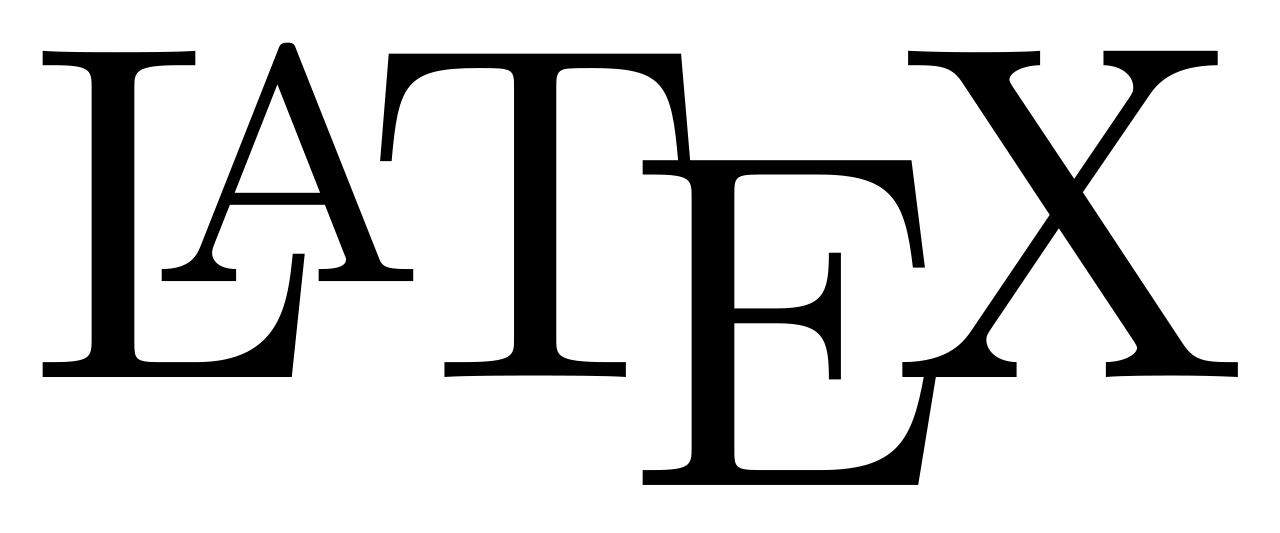
\includegraphics[width=6cm]{immagini/loghi/latex.png}
    \caption{Logo \LaTeX}
\end{figure}
\LaTeX presenta caratteristiche di stabilità e qualità al di sopra dei comuni \emph{wordprocessor}\glsfirstoccur in commercio, soprattutto per quanto riguarda la realizzazione di complesse tabelle o formule matematiche. 
\\
Inoltre, può essere esteso ed ampliato mediante diversi pacchetti. È distribuito con una licenza di software libero e questo lo ha reso disponibile per praticamente qualsiasi architettura: ne esistono pertanto versioni funzionanti per tutti i sistemi operativi, tra cui anche Microsoft Windows, macOS e le varie distribuzioni Linux.

\subsection{Strumenti di analisi statica e dinamica del codice}
\subsubsection{Psalm}
Psalm è uno strumento di analisi statica dedicato all'ambiente di sviluppo PHP che permette di \textit{debuggare} il codice scritto nel linguaggio \textit{serverside} più utilizzato al Mondo. Psalm permette di mantenere alto il livello di qualità del codice, specialmente se condiviso da un gruppo di persone, monitorando e prevenendo gli errori di \textit{runtime}.
\\
Psalm cerca, nella migliore maniera possibile data dal suo algoritmo interno, di interpretare ogni singola riga di codice per scovare svariate tipologie di errore. Oltre a questa caratteristica, tipica degli strumenti di analisi statica e di debugging di codice, Psalm offre funzionalità personalizzate come:
\begin{itemize}
    \item tenere traccia delle operazioni logiche del codice, producendo notifiche nei casi in cui si incontrano determinate asserzioni;
    
    \item controllare che tutte le proprietà di un dato oggetto abbiano un valore assegnato dopo la chiamata alla funzione costruttore
    
    \item supportare une formato che comprende gli array “object like”, permettendo di specificare il tipo delle chiavi degli stessi array.
\end{itemize}

\subsubsection{PHPUnit}
PHPUnit è un framework che oltre a fornire delle interfacce di base per scrivere \textit{Unit Test}, implementa anche una serie di funzionalità aggiuntive estremamente utili che aiutano a scrivere test ben ordinati ed assolutamente efficienti.
\\
PHPUnit si basa sull'idea che gli sviluppatori dovrebbero essere in grado di trovare rapidamente errori nel loro codice appena eseguito e affermare che nessuna regressione del codice si è verificata in altre parti del codice di base. Proprio come gli altri framework di \textit{Unit Test}, PHPUnit utilizza asserzioni per verificare che il comportamento del componente specifico in fase di test si comporti come previsto.
%**************************************************************
\section{Ciclo di vita del software}
\label{sec:ciclo-vita-software}
Il modello adottato per la realizzazione del progetto è quello a spirale in quanto permette di scomporre il processo di sviluppo in quattro fasi multiple, ciascuna ripetuta più volte.
\\
Queste fasi sono:
\begin{itemize}
    \item \textbf{Pianificazione:} nella pianificazione si determinano degli obiettivi, delle alternative e i vincoli associati al progetto. Il committente e il fornitore del sistema interagiscono allo scopo di definire in maniera sufficientemente univoca cosa deve essere realizzato e come. In questa fase è buona norma redigere dei documenti, in principio non eccessivamente dettagliati, che fissino i punti fondamentali della pianificazione del lavoro futuro;
    
    \item \textbf{Analisi dei rischi:} Nell'analisi dei rischi si identificano e si analizzano i problemi e i rischi associati al progetto, al fine di determinare delle strategie per controllarli;
    
    \item \textbf{Sviluppo:} Nella fase di sviluppo si procede alla vera e propria realizzazione: i tempi di realizzazione di questa attività, che comprende sia la codifica sia la verifica, sono tra i più lunghi tra tutti quelli previsti all'interno del ciclo di vita del prodotto software;
    
    \item \textbf{Valutazione:} Nella fase di valutazione il committente valuta se il sistema realizzato risponde alle sue esigenze. Attraverso questa fase il committente verifica che il prodotto soddisfi effettivamente i requisiti richiesti. Una logica conseguenza del fatto che un prodotto software non superi la fase di validazione dei requisiti è la necessità di impostare un nuovo ciclo di attività.
\end{itemize}

%**************************************************************
\section{Progettazione}
\label{sec:progettazione}
    L’architettura generale del software è costituita da un \emph{\textit{frontend}\glsfirstoccur}, da un \emph{\textit{backend}\glsfirstoccur} e da un database che si occupa di mantenere la persistenza dei dati.
    \\
    \\
    Il \emph{\textit{Design pattern}\glsfirstoccur} adottato per la realizzazione dell'applicativo è l'\emph{\textit{MVC}\glsfirstoccur} che è un pattern architetturale molto diffuso nello sviluppo di sistemi software, in particolare nell'ambito della programmazione orientata agli oggetti, in grado di separare la logica di presentazione dei dati dalla logica di business.
    \begin{figure}[!h] 
        \centering 
        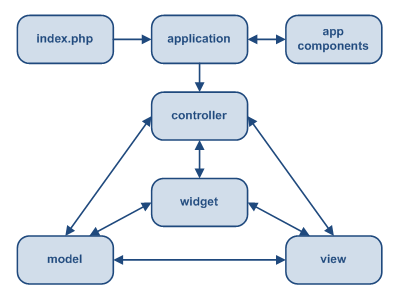
\includegraphics[width=10cm]{immagini/structure.png}
        \caption{Struttura architettura}
    \end{figure}
    \newpage
    Le funzioni del \textit{controller} che hanno lo stesso nome della \textit{view} si occupano della renderizzazione di quest'ultima grazie alla chiamata della funzione \texttt{render(\$view, \$template)} che richiede come parametri il nome della view e il \textit{template} di \textit{view} che si vuole renderizzare. Queste funzioni si occupano anche di restituire alla \textit{view} i dati prelevati mediante apposite \textit{query} contenute nella classe \textit{protocollimodel} nel model.
    
    \subsection{Dashboard}
    Per ottenere la pagina di visualizzazione della lista di protocolli, il più fedele possibile a quanto richiesto, le funzioni da realizzare saranno:
    
    \subsubsection{\texttt{daschboard()}}
    Questa funzione si occupa della renderizzazione della pagina "Dashboard" e si interfaccia con il database mediante la query contenuta in \texttt{getProtocolsToSeeForUser(\$user)} per ricordare all'utente quanti protocolli deve ancora visionare.
    
    \subsubsection{\texttt{getProtocolsForAdmin()}}
    Questa funzione popola la \textit{datatable} nella dashboard di un amministratore che può vedere ed elaborare tutti i protocolli inseriti nel sistema. La stessa si interfaccia con il database mediante la query contenuta nella funzione \texttt{getProtocolsForAdmin()} in \textit{protocollimodel}.
    
    \subsubsection{\texttt{getProtocols()}}
    Questa funzione popola la \textit{datatable} della dashboard di un utente normale che può visionare ed elaborare solo i protocolli a lui attribuiti o da lui inseriti. La stessa si interfaccia con il database mediante la query contenuta nella funzione \texttt{getProtocolliForUsers()} in \textit{protocollimodel}.
    
    %registrazioneprotocollo
    \subsection{Registrazione protocollo}
    Per permettere ad utente di registrare un protocollo le funzioni da realizzare saranno:
    
    \subsubsection{\texttt{protocolRegistration()}}
    Questa funzione si occupa della renderizzazione della pagina "Registrazione Protocollo" e si interfaccia con il database per la generazione automatica di codici progressivi ed univoci quali codice seriale e codice a barre. 
    Le due \textit{query} sono rispettivamente contenute nelle funzioni \texttt{codeGenerator(\$register)} e \texttt{barcodeGenerator()} situate all'interno di \textit{protocollimodel}.
    \\
    La funzione si occupa inoltre di creare un array associativo dei risultati ottenuti dalle \textit{query} contenute nelle funzioni \texttt{getFromDomd()} e \texttt{getFromDprt()}.
    Questo array permette di attribuire ad ogni tipologia di protocollo esistente i suoi corrispettivi metadati.
    
    \subsubsection{\texttt{getSco()}}
    Questa funzione si interfaccia con il database mediante la funzione \texttt{searchSco(\$type, \$search)} che prende come parametri la tipologia di proprietario a cui si vuole intestare il protocollo e la iniziali del nome dell'intestatario del medesimo protocollo. 
    \\
    La stessa è utilizzata per restituire i suggerimenti mediante la funzione che utilizza \textit{EasyAutocomplete} riportata nel paragrafo \hyperref[EasyAutocomplete]{EasyAutocomplete}
    
    \subsubsection{\texttt{nextProtocol(\$register)}}
    Questa funzione viene chiamata al variare della selezione del registro di appartenenza e si occupa di creare un JSON contenente il codice seriale corrispondente al nuovo registro selezionato.
    
    \subsubsection{\texttt{addProtocol()}}
    Questa funzione viene chiamata alla selezione del tasto \textit{submit} e si occupa di salvare nelle rispettive tabelle del database i dati inseriti nel form di registrazione di un nuovo protocollo.
    
    %detailPage
    \subsection{Visualizzazione protocollo}
    Per permettere ad un utente di consultare le informazioni riguardanti un protocollo le funzioni da realizzare saranno:
    
    \subsubsection{\texttt{detailPage(\$serial\_code)}}
    Questa funzione si occupa della renderizzazione della pagina "Dettaglio protocollo" e si interfaccia con il database mediante le seguenti funzioni:
    \begin{itemize}
        \item \texttt{getProtocol(\$protocolcod)} per restituire tutte le informazioni riguardanti il protocollo passato come parametro della funzione;
        
        \item \texttt{getMetadatiPerProtocollo(\$protocolcod)} per restituire tutti i metadati assegnati al protocollo passato come parametro della funzione;
        
        \item \texttt{getAddettiConDataChiusuraAtut(\$typecod, \$serialcode)} per restituire tutti gli operatori assegnati all'elaborazione del protocollo.
    \end{itemize}
    Questa funzione si occupa inoltre di prelevare dall'archivio "F12 Documentale" il documento allegato al protocollo in fase di registrazione del medesimo.
    
    \subsubsection{\texttt{findMatch()}}
    Questa funzione permette di accedere alla pagina di dettaglio di un protocollo mediante lo \textit{scan} di codice a barre. Per fare in modo che ciò avvenga viene chiamata la funzione \texttt{getProtocolFromBarcode(\$barcode)} che mediante \textit{query} preleva dal database il protocollo avente come barcode il codice scansionato.
    
    \subsubsection{\texttt{updateClosingAtut()}}
    Questa funzione permette di aggiornare lo stato di un protocollo quando l'utente dichiara di averlo visionato. Verrà fatto un update del campo dedicato impostando come valore la data e l'ora in cui l'utente ha marcato come visionato tale protocollo.
    
    \subsubsection{\texttt{saveChat()}}
    Questa funzione permette di salvare e visualizzare istantaneamente un messaggio inserito nella sezione "Timeline e Commenti".
    
    %sendMail
    \subsection{Invia e-mail}
    Per consentire l'invio di un protocollo tramite posta elettronica le funzioni da realizzare saranno:
    
    \subsubsection{\texttt{sendMail(\$serial\_code)}}
     Questa funzione si occupa della renderizzazione della pagina "Invia mail" e si interfaccia con il database mediante la funzione \texttt{getIndirizzi(\$codice)} per proporre all'utente gli indirizzi del personale interno o dell'intestatario del protocollo.
    
    \subsubsection{\texttt{send()}}
    Questa funzione viene chiamata alla selezione del tasto "Invia" e si occupa di inviare la mail al destinatario selezionato usando la funzione \texttt{sendMail(\$to, \$from, \$object, \$msg, \$file)}
    
    %typeConfiguration
    \subsection{Registrazione protocollo}
    Per permettere ad un utente la facile consultazione di tipologie esistenti o per crearne di nuove le funzioni da realizzare saranno:
    
    \subsubsection{\texttt{typeConfiguration()}}
    Questa funzione si occupa della renderizzazione della pagina "Configurazione tipologia protocollo" e si interfaccia con il database mediante le seguenti funzioni:
    \begin{itemize}
        \item \texttt{codDotiGenerator()} per la generazione del codice univoco della nuova configurazione;
        \item \texttt{getGruppi()} per restituire come \textit{option} tutti gli uffici esistenti;
        \item \texttt{getUtentiFromGruppo(\$office)} per restituire tutti gli operatori facenti parte dell'ufficio selezionato.
    \end{itemize}
    
    \subsubsection{\texttt{nextGroup()}}
    Questa funzione viene chiamata quando un'utente dichiara di voler aggiungere un nuovo ufficio, con rispettivo personale, addetto all'elaborazione del documento. 
    \\
    Questa si occupa di creare un JSON contenente tutti gli uffici registrati nel database tranne quelli già selezionati.
    
    \subsubsection{\texttt{nextUsers(\$group)}}
    Questa funzione si occupa di creare un JSON contenente tutti gli operatori facenti parte dell'ufficio selezionato.
    
    \subsubsection{\texttt{getConfig()}}
    Questa funzione popola la \textit{datatable} che mostra all'utente tutte le tipologie esistenti. La stessa si interfaccia con il database mediante la query contenuta nella funzione \texttt{getConfiguration()} in \textit{protocollimodel}.
    
    \subsubsection{\texttt{addConfig()}}
    Questa funzione viene chiamata alla selezione del tasto \textit{submit} e si occupa di salvare nelle rispettive tabelle del database i dati inseriti nel form per la creazione di una nuova tipologia di protocollo.
    
    %typeConfigurationDetail
    \subsection{Visualizzazione tipologia}
    Per permettere ad un utente di consultare le informazioni riguardanti una tipologia di protocollo le funzioni da realizzare saranno:
    
    \subsubsection{\texttt{typeConfigurationDetail(\$type\_code)}}
    Questa funzione si occupa della renderizzazione della pagina "Dettaglio configurazione" e si interfaccia con il database mediante le seguenti funzioni:
    \begin{itemize}
        \item \texttt{getMetadati(\$protocolscod)} per restituire tutti i metadati assegnati alla tipologia di cui si sta visionando i dettagli;
        
        \item \texttt{getNumDocumentByTipol(\$protocolscod)} per controllare se nel database ci sono protocolli con la tipologia corrispondente a quella in esame. Questo controllo viene fatto per permettere o meno all'utente di eliminare una tipologia;
        
        \item \texttt{getAddetti(\$protocolscod)} per restituire tutti gli operatori addetti all'elaborazione della tipologia in esame;
        
        \item \texttt{getGroup()} per restituire tutti gli uffici di cui gli operatori addetti fanno parte. 
    \end{itemize}
    
    \subsubsection{\texttt{reset()}}
    Questa funzione viene chiamata alla selezione del tasto "Reset" nella pagina di dettaglio della tipologia e fa la \textit{delete} nel \textit{database} di tutti gli operatori assegnati a quella tipologia.
    
    \subsubsection{\texttt{addNewOperators()}}
    Questa funzione viene chiamata alla selezione del tasto "submit" nella pagina di dettaglio della tipologia e permette di inserire nuovi operatori addetti all'elaborazione della tipologia in esame.
    
    \subsubsection{\texttt{addNewMeta()}}
    Questa funzione viene chiamata alla selezione del tasto "submit" nella pagina di dettaglio della tipologia e permette di inserire nuovi metadati alla tipologia in esame.
    
    \subsubsection{\texttt{deleteConfig()}}
    Questa funzione viene chiamata alla selezione del tasto "Elimina" nella pagina di dettaglio della tipologia e permette di eliminarela configurazione in esame.

%**************************************************************
\section{Codifica}
%**************************************************************
\subsection{Dashboard}

    \subsubsection{Codice}
        Nella pagina denominata \textit{Dashboard} si può visualizzare l'elenco di tutti i protocolli assegnati ad un operatore o registrati dal medesimo operatore.
        \\ 
        L'elenco è stato realizzato utilizzando una \textit{DataTable} ed è popolato mediante \textit{query} che oltre alla \textit{select} dei protocolli si occupa anche dei filtri mediante i quali si può ricercare un protocollo o un gruppo di di protocolli.
        \\
        I filtri sono stati realizzati mediante la concatenazione di condizioni derivanti dall'input dell'utente.
        
        \begin{lstlisting}[language=SQL, caption=Query per Dashboard]
public function getProtocolliForUsers($Dadate, $Adate, $reg, $tipol, $prop, $ope, $fname, $loggedope) {
    $condizione = "";
    if ($Dadate != "")
        $condizione .= " AND dpro_data >= '$Dadate'";
    if ($Adate != "")
        $condizione .= " AND dpro_data <= '$Adate'";
    if ($reg != "")
        $condizione .= " AND dpro_registro = '$reg'";
    if ($tipol != "")
        $condizione .= " AND dpro_tipo = '$tipol'";
    if ($prop != "")
        $condizione .= " AND dpro_nome_prop LIKE '%".strtoupper($prop)."%'";
    if ($ope != "")
        $condizione .= " AND dpro_operatore = '$ope'";
    if ($fname != "")
        $condizione .= " AND dpro_filename_scan LIKE '%$fname%'";

    $sql = "SELECT dpro.*, dprt_descri, dprt_cod_doti  
            FROM dpro, dprt
            WHERE dpro_tipo = dprt_codice
            AND dpro_operatore = '$loggedope' $condizione
            UNION
            SELECT dpro.*, dprt_descri, dprt_cod_doti  
            FROM dpro, dprt, dpru
            WHERE dpro_tipo = dprt_codice
            AND dprt_cod_doti = dpru_codice
            AND dpru_cod_utente = '$loggedope' $condizione
            UNION
            SELECT dpro.*, dprt_descri, dprt_cod_doti  
            FROM dpro, dprt, dpru, usbg
            WHERE dpro_tipo = dprt_codice
            AND dprt_cod_doti = dpru_codice
            AND dpru_cod_gruppo = usbg_group
            AND usbg_operatore = '$loggedope' 
            AND dpru_cod_utente = '' $condizione";
    $res = $this->query($sql);
    return $res;
}
        \end{lstlisting}
        
        
        Il risultato della \textit{query} viene poi elaborato dalla funzione \textit{getProtocols()} che mediante \textit{array} attribuisce ad ogni colonna della \textit{DataTable} il corrispondete valore. 
        \\
        Infine l'\textit{array} viene convertito in formato JSON per essere elaborato dalla \textit{DataTable}.
        \begin{lstlisting}[language=PHP, caption=Funzione getProtocols()]
public function getProtocols(){
    $Dadate='';
    $Adate='';
    $reg='';
    $tipol='';
    $prop='';
    $ope='';
    $fname='';
    foreach ($_REQUEST['filters'] as $filter) {
        if($filter['name']=='Dadata'){
            $Dadate = $filter['value'];
        }
        if($filter['name']=='Adata'){
            $Adate = $filter['value'];
        }
        if($filter['name']=='registro'){
            $reg = $filter['value'];
        }
        if($filter['name']=='tipologia'){
            $tipol = $filter['value'];
        }
        if($filter['name']=='proprietario'){
            $prop = $filter['value'];
        }
        if($filter['name']=='operatore'){
            $ope = $filter['value'];
        }
        if($filter['name']=='filename'){
            $fname = $filter['value'];
        }
    }
    $protocolli = $this->model->getProtocolliForUsers($Dadate, $Adate, $reg, $tipol, $prop, $op$fname, $_SESSION[NOME_SESSIONE]['user']);
    $return['data'] = array();
    $i=0;
    foreach($protocolli as $p) {
        $return['data'][$i]['DT_RowId'] = $p->dpro_serial_doc;
        $return['data'][$i][0] = $p->dpro_serial_doc;
        $return['data'][$i][1] = $p->dpro_filename_scan;
        $return['data'][$i][2] = $p->dprt_descri." (".$p->dprt_codice.")";
        if ($p->dpro_registro == 'S'){
            $return['data'][$i][3] = "Spedito";
        } elseif ($p->dpro_registro == 'R'){
            $return['data'][$i][3] = "Ricevuto";
        } else {
            $return['data'][$i][3] = "Interno";
        }
        $return['data'][$i][4] = $p->dpro_operatore;
        $return['data'][$i][5] = $p->dpro_data;
        $return['data'][$i][6] = $p->dpro_barcode_tag;
        $return['data'][$i][7] = $p->dpro_nome_prop;
        $i++;
    }
    echo $this->mw_json_encode($return);
}
        \end{lstlisting}
        
    \subsubsection{Resa finale}
        È stata prestata molta attenzione alla presentazione grafica della pagina, cercando un'estetica semplice ma professionale.
        
        \begin{figure}[!h] 
            \centering 
            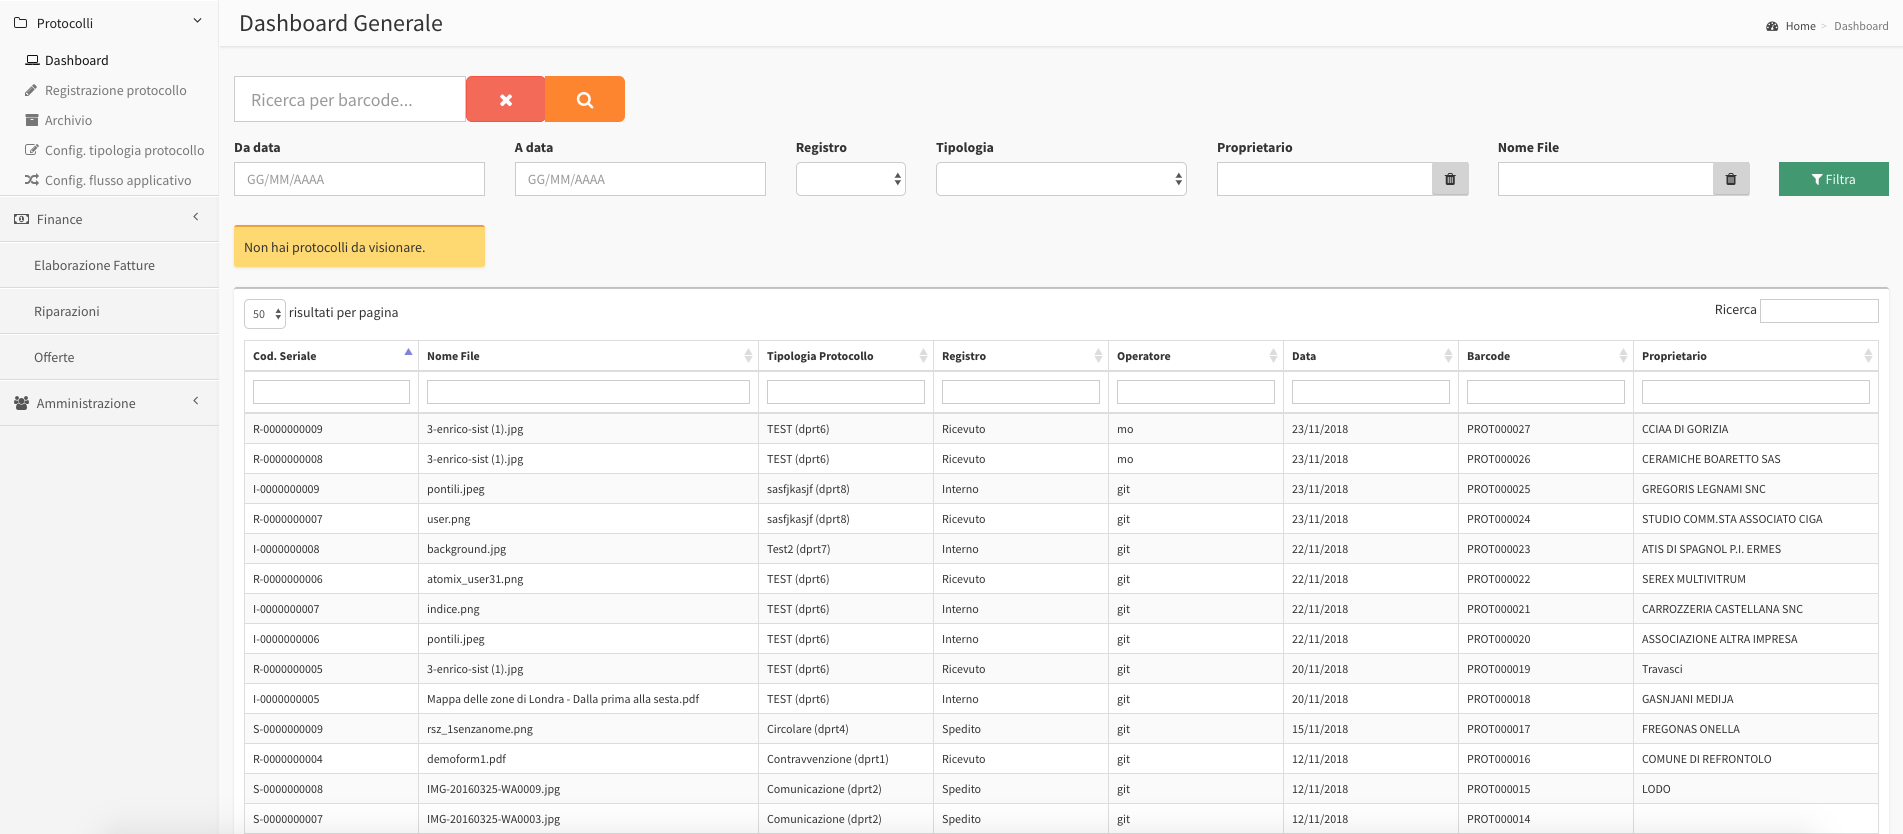
\includegraphics[width=\textwidth]{immagini/prodottofinito/dashboard.png}
            \caption{Dashboard view}
        \end{figure}
        \newpage
        L'\textit{header} della pagina è dedicata ai filtri. 
        \\
        Come richiesto dal requisito \hyperref[RFO6]{RFO6} sarà possibile, mettendo il \textit{focus} sul campo \textit{input} nominato "Ricerca per \textit{barcode}", accedere direttamente al dettaglio del protocollo di cui si è effettuato lo \textit{scan} del \textit{barcode}.
        \\
        Al di sotto di questo campo l'utente potrà filtrare i protocolli per tutti i campi visibili della \textit{DataTable}.

\subsection{Visualizzazione Protocollo}

    \subsubsection{Codice}
        Nella pagina di visualizzazione di un singolo protocollo oltre alle informazioni generali prelevate dal database mediante apposita \textit{query} viene inoltre presentata una preview del documento protocollato.
        \\
        Essendo il documento salvato nella piattaforma documentale "F12 Documentale", per essere stampato a video, bisogna seguire i seguenti \textit{step}:
        \begin{itemize}
            \item comporre il link dove il documento è contenuto;
            
            \item estrarre il contenuto del link appoggiandosi alla funzione \textit{file\_get\_contents()};
            
            \item decodificare il risultato JSON ottenuto;
        
            \item creare una cartella temporanea dove salvare temporaneamente il file d'interesse;
            
            \item creare la view per stampare il file in base alla tipologia dello stesso.
        \end{itemize}
        
        \begin{lstlisting}[language=PHP, caption=Pint della preview del documento]
//URL
$pathpreview = $this->model->getWSPathDocu('preview');
$wsdocupath = $pathpreview."/".$this->protocollo->dpro_docu_id."/";
    
//PERNDO IL CONTENUTO DELL'URL
$target = file_get_contents($wsdocupath);
    
//DECODE
$docs = json_decode($target);
$decoded = base64_decode($docs->doc);
    
    
//PRELEVO LE INFORMAZIONI DI INTERESSE
$mime = $docs->mime;
$name = $docs->name;
$this->desc = $docs->docd_descriz;
    
$this->pathdocumentotmp = SERVER_ROOT.'/files/tmp/'.$name;
    
if(!is_dir(SERVER_ROOT.'/files/tmp/')){
    $this->model->mw_mkdir(SERVER_ROOT.'/files/tmp/');
}
    
//IN BASE AL FILE DIVERSI TIPI DI VIEW
file_put_contents($this->pathdocumentotmp, $decoded);
$ppp = '';
if (exif_imagetype($this->pathdocumentotmp) != false) {
    $ppp.= '<div class="imagecontainer">';
    $ppp.= '<img style="width:100%;" src="' . SITE_ROOT.'/files/tmp/'.$name . '" >';
    $ppp.= '</div>';
} else if ($mime == 'application/pdf') {
    $ppp.= '<div class="imagecontainer">';
    $ppp.= '<iframe src="' . SITE_ROOT.'/files/tmp/'.$name . '" width="100%" height="600" ></iframe>';
    $ppp.= '</div>';
} else {
    $ppp.= '<div class="imagecontainer">';
    $ppp.= '<img id="myImg" style="width:100%;" src="' . SITE_ROOT . '/files/img/PNA.png" >';
    $ppp.= '</div>';
}
$this->prev = $ppp;
        \end{lstlisting}
    
    \subsubsection{Resa finale}
        \begin{figure}[!h] 
            \centering 
            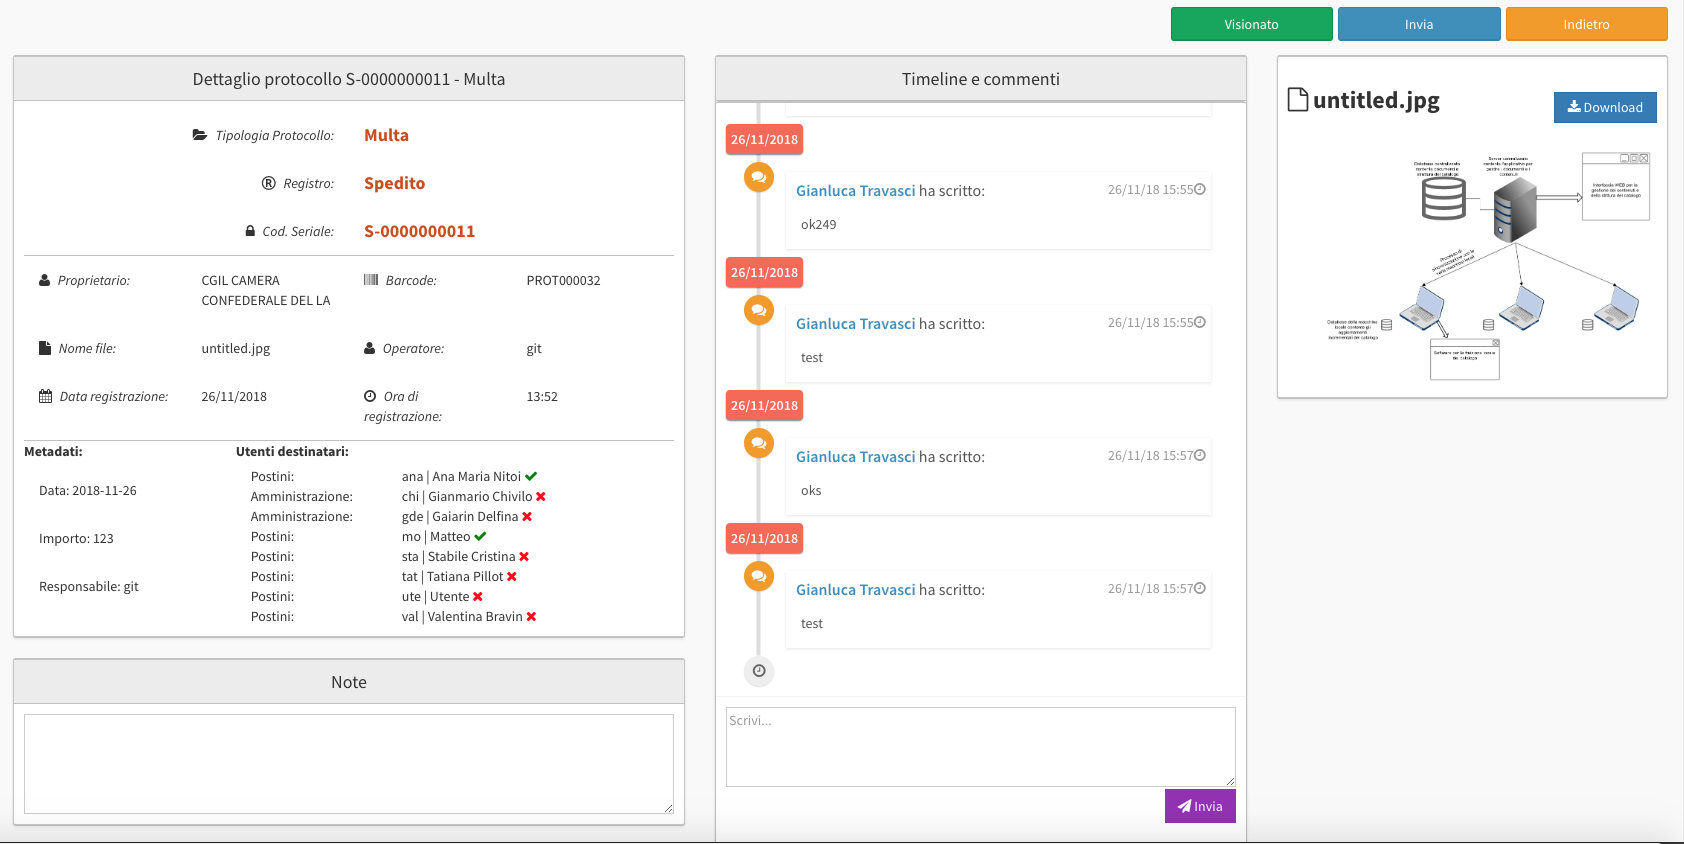
\includegraphics[width=\textwidth]{immagini/prodottofinito/dettproto.png}
            \caption{Dettaglio protocollo view}
        \end{figure}
       
        L'immagine in \textit{preview} è scaricabile mediante apposito bottone che si collega all'url per il download del documento sulla piattaforma "F12 Documentale".
        \\
        Ogni volta che viene registrato un protocollo viene creata una riga, per ogni utente coinvolto, nell'apposita tabella del \textit{database} con campo "chiusura \textit{task}" impostato di \textit{default} a null.
        \\
        Quando l'operatore asserisce di aver visionato il documento, premendo il bottone "Visionato", il campo "chiusura task" verrà aggiornato con la data e l'ora corrente e accanto al proprio nome comparirà una spunta verde.
        \\
        Questo salvataggio della data e dell'ora permette inoltre di tenere traccia dello storico del documento come richiesto dal requisito \hyperref[RFO3.1.11]{RFO3.1.11}.
        
\subsection{Registrazione Protocollo}
    \subsubsection{Codice}
        Al variare della tipologia di documento selezionata vengono stampati a video i campi metadato creati in fase di configurazione della tipologia. Per realizzare tale funzionalità è stata creata una \textit{query} che preleva dalla tabella dedicata ai metadati tutti quelli corrispondenti alla tipologia selezionata, quindi mediante script è stata eliminata la \textit{html class} che settava a \textit{"display: none"} e rendeva nascosti tali campi input.
        \\
        Lo stesso principio è stato adottato per la selezione della "Tipologia proprietario" e del "Nome Proprietario" nel caso in cui si selezioni "Nuovo Contatto".
        In questo caso, in fase di salvataggio, il valore del campo "Nome e Cognome (Azienda)" verrà salvato nella tabella delle informazioni sul protocollo sotto la voce "Nome Proprietario"
        \\
        Tutti i dati inseriti e visualizzati non modificabili, un volta premuto il bottone \textit{submit} della form di registrazione di un nuovo protocollo, vengono passati tramite una richiesta POST e sono disponibili lato server nella variabile \$\_POST. In seguito i dati vengono memorizzati nel database appoggiandosi alla funzione \textit{insert(\$dati, \$tabella)} presente nel \textit{framework} aziendale.
        \\
        Il documento caricato in fase di compilazione della form viene trasmesso mediante cURL al servizio "F12 Documentale" in cui verrà archiviato. 
       \newpage \begin{lstlisting}[language=PHP, caption=Upload su Documentale]
$pathdoc=$this->model->getPathDoc();
$urlpath = str_replace("/documentale/documentale/documentif12/","/documentale_coop/documentale/uploadfile", $pathdoc);
$url = $urlpath."?mask=".$funzione_accesso."&val=".$_POST['dpro_serial_doc']."&ope=".$_SESSION[NOME_SESSIONE]['user']['sigla']."&rowval=&db=dbf12&tipologia=".$_POST['dpro_tipo']."&external=1";

foreach($_FILES as $nome => $file) {

    if (trim($file['name']) != "") {
        $desc = isset($_REQUEST['desc']) ? $_REQUEST['desc'] : '';
        $curl = curl_init();

        $post_data = array('file' => '@' . $file['tmp_name'], 'name' => $file['name'], 'type' =$file['type'], 'dsc' => $desc);
        curl_setopt($curl, CURLOPT_POSTFIELDS, $post_data);

        // OPTIONS:
        curl_setopt($curl, CURLOPT_URL, $url);
        curl_setopt($curl, CURLOPT_RETURNTRANSFER, 1);
        curl_setopt($curl, CURLOPT_SSL_VERIFYPEER, false);

        // EXECUTE:
        $result = curl_exec($curl);
        curl_close($curl);
    }
}
        \end{lstlisting}
        Sulla variabile \textit{\$result} viene salvato il codice univoco della riga del database corrispondente al documento caricato. Il codice viene poi usato per fare l'\textit{update} del campo \textit{id\_documentale} nella riga della tabella dedicata alle informazioni del protocollo mettendo così le due tabelle in relazione "uno a uno".
    \subsubsection{Resa finale}
        \begin{figure}[!h] 
            \centering 
            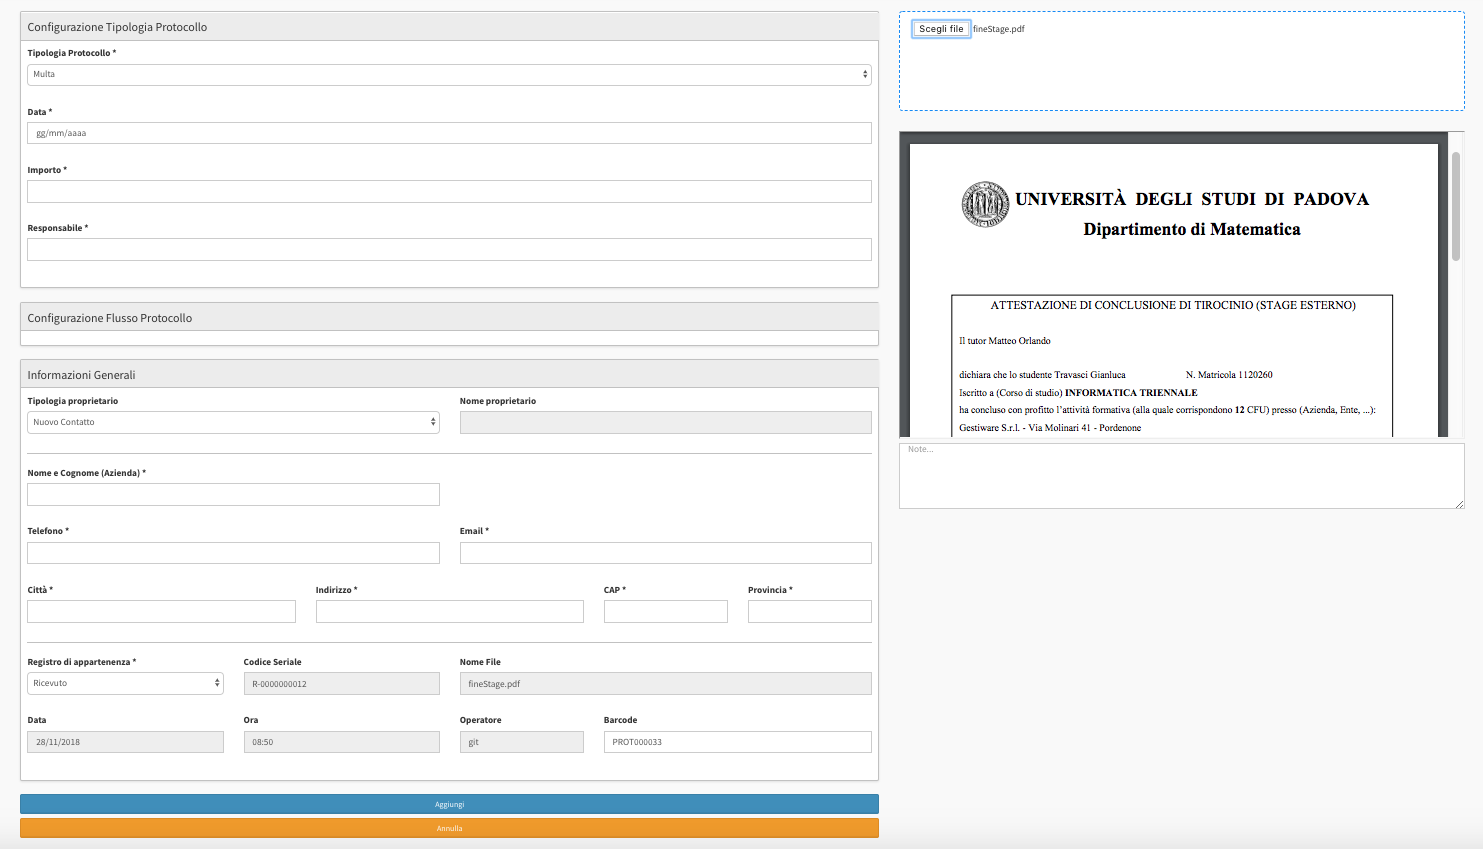
\includegraphics[width=\textwidth]{immagini/prodottofinito/regproto.png}
            \caption{Registrazione protocollo view}
        \end{figure}
        Come accennato precedentemente, selezionando "Nuovo Contatto" nella selezione della "Tipologia proprietario" il campo "Nome Proprietario" verrà disabilitato e comparirà la form di registrazione di un nuovo contatto.
        
\subsection{Configurazione della tipologia}
    \subsubsection{Codice}
        Come precedentemente descritto per la dashboard, per presentare tutte le tipologie esistenti è stata adottata una \textit{DataTable}.
        \\
        Per l'assegnazione degli operatori addetti all'elaborazione della tipologia di protocollo in fase di creazione sono state utilizzate due chiamate \textit{Ajax}.
        \\
        La prima è stata realizzata per far fronte all'esigenza di poter aggiungere utenti facenti parte di diversi uffici. Quando viene assegnato il primo ufficio con rispettivo personale e viene premuto il tasto "Aggiungi" viene effettuata la chiamata \textit{Ajax} e se essa ha successo viene fatto l'\textit{append} di una nuova riga di codice html.
        \\
        I dati da stampare nelle select vengo passati in formato JSON dalla funzione apposita nel \textit{controller} e vengono decodificati mediante funzione \textit{parseJSON(data)}.
        \\ 
        Premendo il tasto "Elimina" verrà eliminata la nuova riga aggiunta.
        \begin{lstlisting}[language=PHP, caption= JQuery per nuova riga]
var i=1;
$('#addgruppo').click(function(){
    i++;
    $.ajax({
        url: baseurl+'/protocolli/nextGruppi',
        success: function (data) {
            var parsed = $.parseJSON(data);
            console.log(parsed.gruppinext);
            var html='<div id="row'+i+'">' +
                    '<div class="col-md-5">'+
                        '<select class="form-control gruppi-esistenti required" id="'+i+'" name="gruppi[sezione][]">' +
                            '<option></option>';
                            $.each(parsed.gruppinext,function (i,v) {
                                    html+= '<option value="'+ v.uswg_codice +'">'+ v.uswg_descrizione +'</option>'
                            });
                        html += '</select>'+
                    '</div>' +
                    '<div class="col-md-5">'+
                        '<select class="form-control operatori-da-attribuire required" id="'+i+name="gruppi[contatti][]">' +
                            '<option></option>' +
                            '<option value="T">Tutti</option>' +
                            '<option value="S">Seleziona</option>' +
                        '</select>' +
                        '<div class="row hide" id="operatori-assegnabili-'+i+'">' +
                            '<div class="box box-nomi-'+ i +'" style="margin-top: 1em; padding-left: 5px;">' +
                            '</div>'+
                        '</div>'+
                    '</div>'+
                    '<div class="col-md-2">' +
                            '<button type="button" name="remove" id="'+i+'" class="btn btn-danger btn_remove_gruppo">Elimina</button>' +
                    '</div>' +
            '</div>';
            $('#aux').append( html );
        }
    });
});
$(document).on('click', '.btn_remove_gruppo', function(){
    var button_id = $(this).attr("id");
    $('#row'+button_id+'').remove();
});
        \end{lstlisting}
        
        La seconda chiamata \textit{Ajax} è stata realizzata per far fronte all'esigenza di poter selezionare solo alcuni utenti facenti parte di un ufficio. 
        \\ 
        Come nel caso della chiamata precedete i dati sono prelevati in formato JSON e sono decodificati con la funzione \textit{parseJSON(data)}.
        \\
        Se la chiamata \textit{Ajax} ha successo viene fatto l'\textit{append} di codice alla classe \textit{box-nomi} e il suddetto box viene visualizzato o meno in base all'opzione selezionata nella \textit{select} "Assegna Utenti".
        \begin{lstlisting}[language=PHP, caption= JQuery Nuovi utenti]
$(document).on('change','select.operatori-da-attribui',function() {
    var id = $(this).attr('id');
    if ($(this).val() == 'S') {
        $('#operatori-assegnabili-'+ i+'').removeClass('hide');
    } else {
        $('#operatori-assegnabili-'+ i+'').addClass('hide');
    }
});
            
$(document).on('change','select.gruppi-esistenti',function(){
    var select_id = $(this).attr("id");
    var get=$(this).val();
            
    $.ajax({
        url: baseurl+'/protocolli/nextUtenti/'+get,
        success: function (data) {
            var parsed = $.parseJSON(data);
            console.log(parsed.utentinext);
            var html='<div>';
            $.each(parsed.utentinext,function (i,v) {
                html+='<div class="row">' +
                    '<div class="col-md-1">' +
                     '<input type="checkboxclass="ablename="operatore-da-assegnare[]value=" '+ v.usbg_operatore +'">+
                    '</div>' +
                    '<div class="col-md-9">' +
                        '<label>'+ v.usbg_operatore +| '+ v.op_nome_op +'</label>' +
                    '</div>' +
                '</div>'
            });
            html+='</div>';
            
            $('.box-nomi-'+ select_id +'').html ( htm);
        }
    });
});
        \end{lstlisting}
       
    \subsubsection{Resa finale}
        \begin{figure}[!h] 
            \centering 
            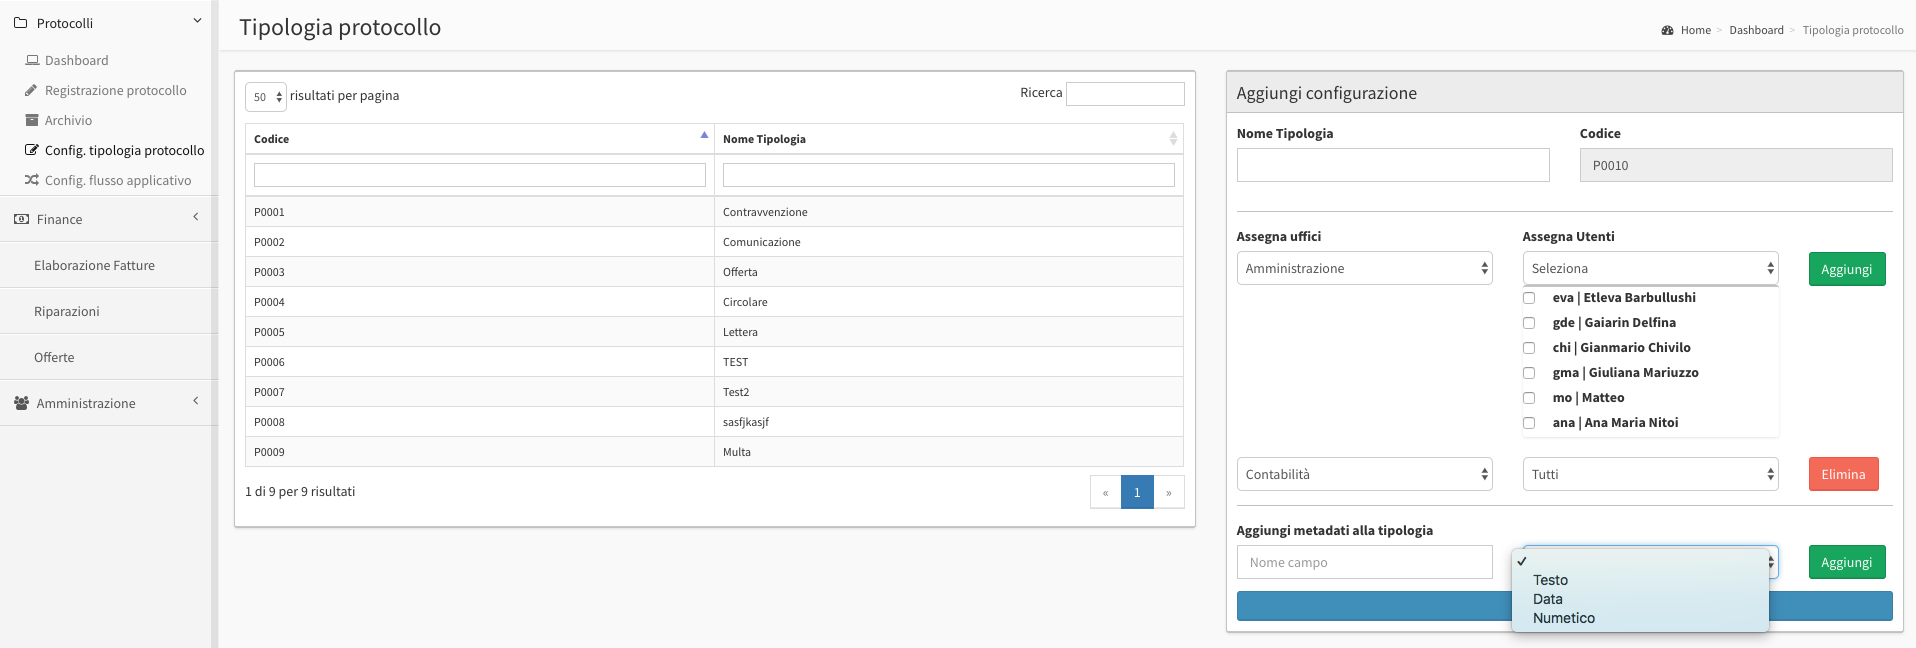
\includegraphics[width=\textwidth]{immagini/prodottofinito/configtipo.png}
            \caption{JQuery per selezione utenti}
        \end{figure}
        Con la precedente immagine è più facile visualizzare quanto precedentemente descritto.
        \\
        Lo stesso principio utilizzato nelle chiamate \textit{Ajax} precedentemente descritte è stato usato per aggiungere metadati a sostegno di una più arricchita descrizione della tipologia in fase di registrazione di un protocollo.
        
\subsection{Visualizzazione tipologia protocollo}
    \subsubsection{Codice}
        Dal punto di vista del codice non c'è nulla di nuovo rispetto alle pagine precedentemente descritte.
        \\
        I dati precedentemente inseriti vengono ora prelevati mediante apposta \textit{query} e stampati a video.
        \\
        È inoltre possibile modificare la configurazione dal punto di vista dei metadati utilizzando lo stesso sistema spiegato per la pagina precedente. 
        \\
        Per quanto riguarda gli operatori addetti, ad ogni modifica per un ufficio già esistente nella lista degli uffici coinvolti viene fatta una \textit{delete} di tutti gli operatori precedentemente inseriti e vengono caricati nel database quelli nuovi.
    \subsubsection{Resa finale}
        \begin{figure}[!h] 
            \centering 
            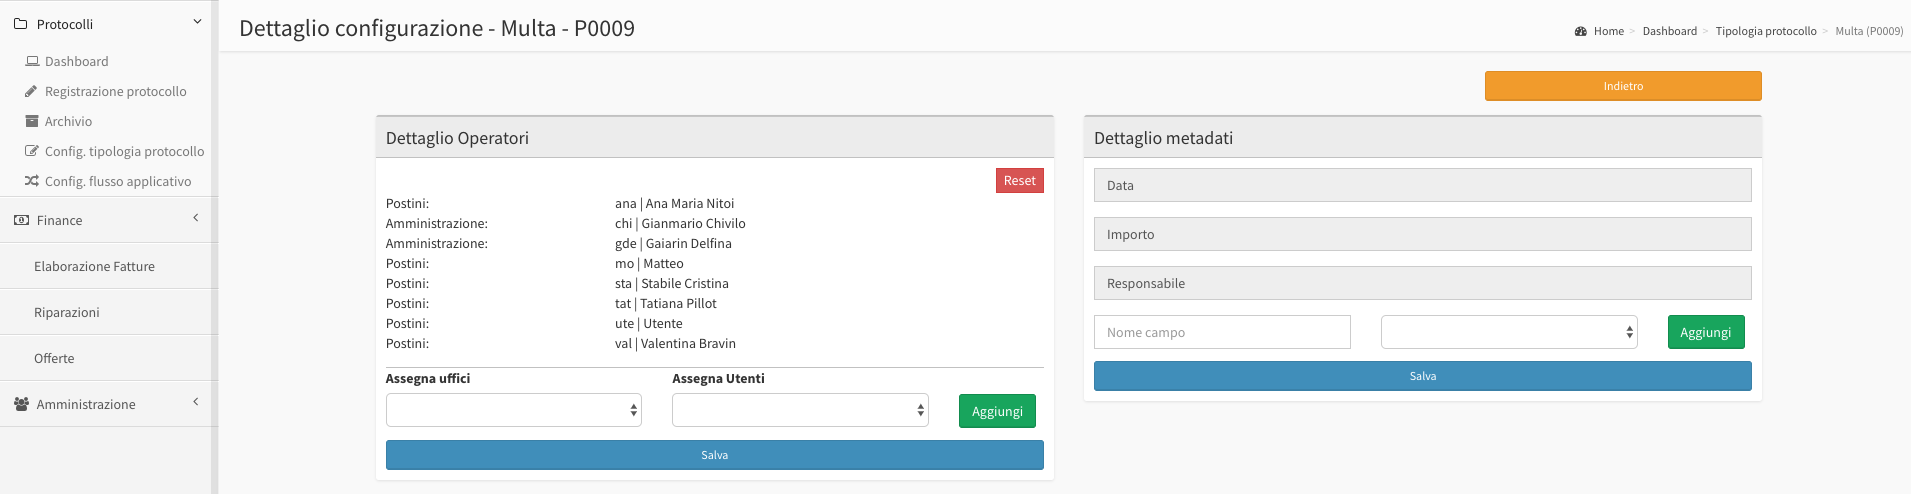
\includegraphics[width=\textwidth]{immagini/prodottofinito/dettaglioconfig.png}
            \caption{Dettaglio configurazione view}
        \end{figure}
        Con il tasto "Reset" è possibile eliminare tutti i gli operatori assegnati per poter riconfigurare da zero la tipologia. 
        \\ 
        Nel caso in cui non vi siano documenti collegati alla tipologia presa in esame, accanto al tasto "Indietro", sarà possibile visualizzare il tasto "Elimina" che consente l'eliminazione della tipologia creata. 
        
        
